\begin{sidewaysfigure}
  \centering
  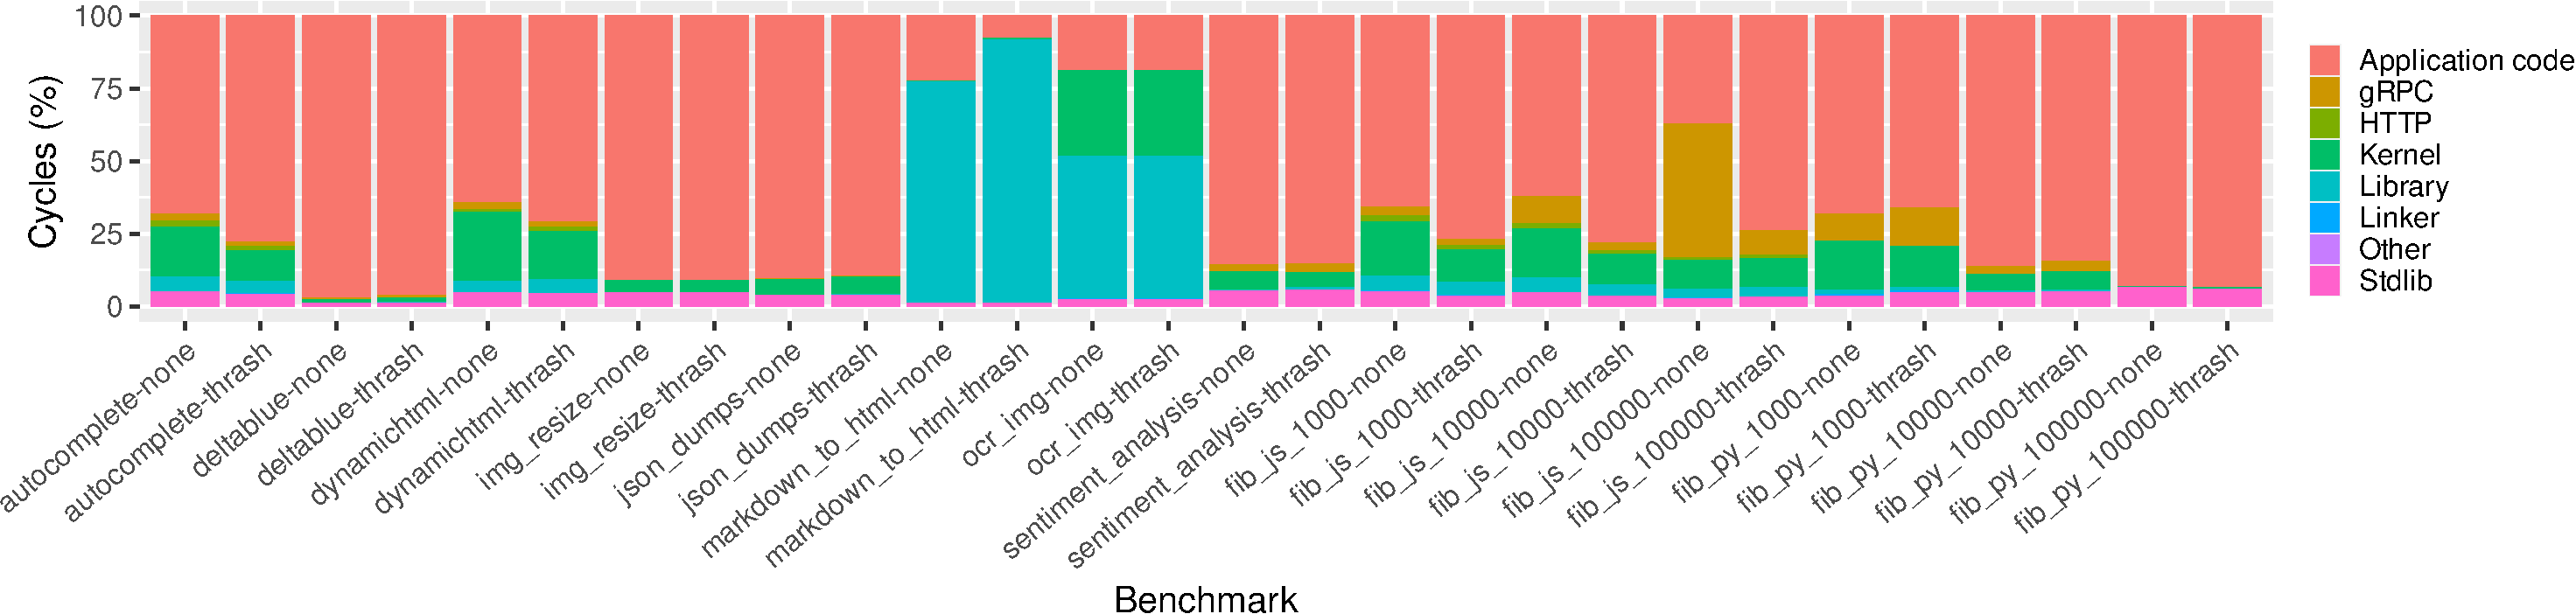
\includegraphics[width=\textwidth]{figures/cycles_per_component.pdf}
  \caption{\label{fig:cyc_per_component} The breakdown of where executed cycles are spent divided into categories.}
  \Description{Stacked bar chart showing the distribution of CPU cycles across application stack components.}
\end{sidewaysfigure}

\begin{table}
    \caption{\label{tab:functions} The functions used for characterization.}
    \resizebox{\textwidth}{!}{
\begin{tabular}{lllll}\toprule
  Name & Language & Description \\\midrule
  autocomplete & NodeJS & Returns a list of autocomplete candidates. \\
  sentiment\_analysis  & Python & Identifies the sentiment of a text. \\
  deltablue & Python  & Pure-python compute benchmark. \\
  markdown2html & Python & \parbox[t]{6cm}{Converts markdown to HTML. Relies heavily on the sha256 implementation in the OpenSSL library.} \\
  json\_dumps & Python & Serializes a Python dict as JSON \\
  img-resize & NodeJS, libraries & \parbox[t]{6cm}{Produces resized versions of images. All of the heavy-lifting in this function is done by native image libraries such as libpng and libjpeg} \\
  ocr-img & NodeJS, C++ & Invokes Tessarect to OCR an image \\
  dynamichtml & NodeJS & Generates HTML from a template  \\
  fib\_js\_NNN & NodeJS & \parbox[t]{6cm}{calculates the NNN'th fibonacci number\\ and returns it}  \\
  fib\_py\_NNN & Python & Same as fib\_js but implemented in Python. \\
  footprint\_NN & Python, C & \parbox[t]{6cm}{Synthetic function that claims a code footprint of NN KB.} \\
  \bottomrule
\end{tabular}}
%\vspace{-4em}
\end{table}


\section{Methodology}
\label{sec:label}

    \subsection{Experimental setup}
We perform our experiments on a server with a 4-core 3.8GHz Intel Xeon E3-1275 v6 (Kaby Lake) processor. The processor has 8MB of shared LLC, 256KB private L2, and 32KB each of private L1-I and L1-D cache and has 64GB of DRAM, SSD drives and both the host system and the application containers run Fedora Linux 36. SMT and Turbo Boost were disabled during the experiments.

Each of the target functions are run inside a Podman container which is pinned to a single processor core. The functions are wrapped by a gRPC server that invokes the function on request. Since the process executing the functions runs as a daemon, as opposed to running as multiple processes, the microarchitectural state is shared across contiguous invocations of the same function. The functions are invoked by a client, implemented in Go, that issues gRPC requests. Each gRPC request only triggers a single invocation and thus, where required by the experiment, the client is configured to repeatedly issue requests for a set amount of time. The client is pinned to a different processor core than the functions. Before statistics collection starts, the functions are warmed by repeated invocations for 30 seconds. This is done to ensure that caches in the execution path are warmed up and that JIT compiled functions had time to reach a fixpoint. Then, the experiments are run for 300 seconds with data collection. The exception to this is the instruction working set estimation (\Cref{subsec:footprint}) which is run only for 30 seconds due to the large amount of data collected. All of the invocations of a single benchmark use the same input data.

To simulate how a function is affected by interleaved execution, we invoke a \emph{thrasher} process between subsequent invocations of a function. The container hosting the thrasher process is pinned to the same processor core as the function and is invoked by the client through a gRPC request after every invocation of the function. Upon invocation, the thrasher performs two operations. First, it fills the BTB and branch predictor with garbage using a process \cite{serverless_state} that executes a long series of conditional and unconditional jumps. Then, to clear caches, it invokes the WBINVD x86 instruction that writes back and invalidates the entire cache hierarchy (L1 to LLC).

To avoid unintentionally collecting data from the thrasher process we configure \texttt{perf} to filter events not belonging to the \texttt{cgroup} of the container running the function.

The evaluated functions are executed in two different configurations. In both cases, function executions happen as fast as possible depending on the function. To distinguish these, we use a consistent naming scheme when presenting our results where the experiment configuration is indicated by a suffix added to the benchmark name as follows:
\begin{description}
\item[Back-to-back]  (\textit{benchmark\_name} suffix \textit{-none}) Each benchmark is repeatedly invoked by back-to-back requests.
\item[Thrashing] (\textit{benchmark\_name} suffix \textit{-thrashing})  The thrasher (as described above) is invoked after each invocation of the function.
\end{description}


\subsection{Function description}
\label{subsec:work_desc}
To perform our experiments, we use a mix of representative and synthetic functions written in Python and NodeJS, the two most popular application runtimes for serverless applications \cite{serverless_state}. A description of the functions and their implementation is provided in \Cref{tab:functions}. The functions used are mainly derived from the FaaSProfiler framework \cite{shahrad19_archit_implic_funct_servic_comput} but we use a custom setup for invoking the functions. As mentioned, we also introduce two synthetic functions to the suite in addition to the representative functions. One, \emph{fib\_js} and \emph{fib\_py} calculates the Nth Fibonacci number and the other, \emph{footprint}, hogs a configurable instruction working set while it is running. \emph{Footprint} achieves this by executing a sequence of jumps to randomized locations in its instruction working set. The Fibonacci calculation function is implemented in both Python and NodeJS allowing us to directly compare the runtime behavior of these two platforms. Since the runtime characteristics of the synthetic functions change depending on their invocation parameters, we use them to corroborate hypotheses derived from the behavior of the representative functions. The observed execution times of the functions are shown in \Cref{tab:timings}.

\label{subsec:footprint}



%%% Local Variables:
%%% mode: latex
%%% TeX-master: "main"
%%% End:
